\documentclass[12pt,fleqn]{article}\usepackage{../../common}
\begin{document}
Ders 1-8

Yaylar ve Agirliklar (Springs and Masses)

Dersimizin uygulama kismina geldik. Diyelim ki alttaki gibi bir yay sistemi var,
4 tane yay 3 tane agirliktan olusuyor, ve sonlari duvar, tavan gibi bir yerde
sabitlenmis.

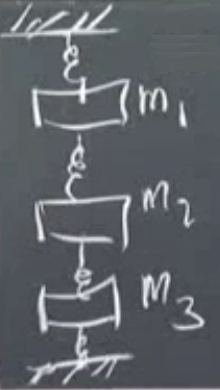
\includegraphics[width=5em]{compscieng_1_08_01.png}

Kutlelerin bir agirligi var tabii, agirliklar o yaylar asagi dogru cekiyor, bu
cekim yaylari acacak, gerecek, soru yaylarin ne kadar asagi inecegi.  Bir yer
degisim (displacement) sorusu bu yani. Unutmayalim yay acilip kapanan bir
mekanizmadir ama acilirken de kapanirken de bir direnc gosterir. Yer degisim en
ustte ve en altta sifir cunku oralar sabitlenmis.

Bir baslangic hali dusunursek, diyelim ki yercekimi o anda etkisiz, ama sonra
yercekimini bir dugmeye basip aciyoruz, her yay baslangic halinden asagi
dogru bir yer degisimi yasayacak, 

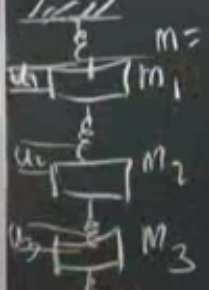
\includegraphics[width=5em]{compscieng_1_08_02.png}

bunlara $u_1,u_2,u_3$ diyebiliriz.

Dikkat salinimi olcmeye ugrasmiyoruz burada, o daha sonraki derslerde devreye
girecek, zaman faktorunu resme dahil edecegiz, o sonra. Simdi sadece kalici
durumla ilgileniyorum, yercekimi aciliyor, yaylar asagi dogru uzuyor, ve her sey
yerli yerine oturduktan sonra gozlemlenecek yer degisimiyle ilgileniyorum su
anda.

Her yay parcasinin ne kadar uzadigi / esnedigi (elongation) ayri bir olcut.
Dusunursek ikinci kutledeki yer degisimi $u_2$ icinde hem ikinci hem de birinci
yayin esnemesi rol oynar. O yuzden esneme icin ayri bir degisken kullaniyoruz,
$e_1,e_2,e_3$. O zaman kinci yay ne kadar uzar? $u_2-u_1$ kadar. Bir farktan
bahsediyoruz burada. Bazi yaylar sikisma da yasayabilir tabii, mesela tahmin
ediyorum ki en alttaki yayda sikisma olacak.

Tum bunlar isin geometrik kismi bir anlamda, yer, uzama, kisalma.. Materyel
faktorlere resme dahil etmek lazim, Hooke Kanunu bunu yapacak. Ilk agirlik
mesela asagi inerken ilk yayi gerecek. Hooke Kanunu bu noktada der ki yay belli
bir kuvvetle agirligi geri cekecek, bu cekis yayin gerilmesi / uzamasiyla
orantili olacak. Her yaydaki kuvvete $w_1,w_2,w_3,w_4$ diyelim. Esneme ile ona
karsilik ortaya cikan kuvvet iliskisi her materyel icin farkli olur, materyele
gore, yay cesidini gore degisen Hooke yay sabiti bu farkliligi denkleme dahil
edebilir, bu sabitlere $c_1,c_2,c_3,c_4$ diyelim.

Hooke Kanunun lineerdir, ki asiri fazla olmayan esnemeler icin lineerlik
gecerli olacaktir, muhakkak yayi asiri gerseydik belli bir noktadan sonra
lineer olmayan etkiler gorebilirdik, biz bu tur asiri sonuclara su anda
bakmiyoruz.

Devam edelim, Hooke Kanunu der ki her yaydaki kuvvet o yaydaki esnemeyle orantilidir,

$$
w_i = c_i e_i 
$$

Burada bir kosegen matris goruyorum ben, tum yaylar, esnemeler, sabitler icin

$$
\left[\begin{array}{c}
w_1 \\ w_2 \\ w_3 \\ w_4
\end{array}\right] =
\left[\begin{array}{cccc}
c_1 & & & \\  & c_2 & & \\  & & c_3 & \\ & & & c_4
\end{array}\right]
\left[\begin{array}{c}
e_1 \\ e_2 \\ e_3 \\ e_4
\end{array}\right] 
$$

Ve nihai matris formunda

$$
w = C e
$$

ki $w,C,e$ ustte gorulen vektorler ve matris. Materyel kismi bu sekilde dahil
etmis olduk, ortadaki sabit matrisi uzerinden. Benzer kanunlar fizigin diger
kisimlarinda da gorulebilir, mesela ustteki $C$ matrisi iletkenligi de temsil
ediyor olabilirdi. Demek istedigim materyel ozellikleri denkleme oradan dahil
oluyor. Bu resmi nasil tamamlariz? Yercekim bir dis kuvvet, kutleler var, yer
degisimlerine sebep oluyor..

Resmi tamamlamak icin ``kuvvet denge'' denklemi ekleyecegim, her kutle
icin bir denge denklemi olacak.

Not ekleyelim, ustteki turden problem modellemesi pek cok diger uygulamada ise
yariyor. Bir geometri var, buradan bir $A$ matrisi cikartiyoruz, sonra bir
fiziksel adim var, oradan $C$ matrisi geliyor, ve kuvvet dengesi ekleniyor,
resim tamamlaniyor. Kuvvet denge denklemi diger bir alanda, mesela elektrikte,
Kirchoff Akim Kanunu olabilirdi, ileride ag yapilarina bakarken gorecegiz, giren
akim cikan akima esit.. Buradaki denge bir yandaki kuvvetin diger yandakine esit
olmasi. Eger sistemde bir dengeden (equilibrium) bahsedebiliyorsak bir denge
denklemi yazabiliriz demektir.

Simdi esneme kismini matris formuna cevirelim. Ne demistik? Mesela ikinci yay
esnemesi ikinci yer degisimi eksi birinci yer degisimi. Matrissel formda
konusmak icin $e_i$ ve $u_j$  vektorlere lazim, iliskileri bir matris carpimi.
Alttaki matriste ikinci satira ne yazariz?

$$
\left[\begin{array}{c}
e_1 \\ e_2 \\ e_3 \\ e_4
\end{array}\right] =
\left[\begin{array}{cccc}
 & & \\ ? & ? & ? \\  & & \\  & & 
\end{array}\right]
\left[\begin{array}{c}
u_1 \\ u_2 \\ u_3 
\end{array}\right]
$$

O satir sagdaki $u$ vektoru ile carpilip sonuclari toplanacak, o zaman
$u_1$ eksi bir ile, $u_2$ arti bir ile carpilir, $u_3$ ile ilgilenmiyoruz,
orasi sifir, yani

$$
\left[\begin{array}{c}
e_1 \\ e_2 \\ e_3 \\ e_4
\end{array}\right] =
\left[\begin{array}{cccc}
 & & \\ -1 & 1 & 0 \\  & & \\  & & 
\end{array}\right]
\left[\begin{array}{c}
u_1 \\ u_2 \\ u_3 
\end{array}\right]
$$

Ustte gorulen satir bu tur matrislerde tipik bir satirdir. Peki birinci
satir neye benzer? Orada sadece $u_1$ olur, tabii $u_1 - u_0$ farki
ama ilk yay en ustte sabitlendigi icin orada yer degisim olmasi mumkun
degil $u_0 = 0$, geriye sadece $u_1$ kaliyor.

Ucuncu satir kolay. Dorduncu satirda $u_4$ sabitlenmis yani sifir,
tek kalan $-u_3$. Hepsi bir arada,

$$
\left[\begin{array}{c}
e_1 \\ e_2 \\ e_3 \\ e_4
\end{array}\right] =
\left[\begin{array}{rrrr}
1 & 0 & 0 \\ -1 & 1 & 0 \\ 0 & -1 & 1 \\ 0 & 0 & -1
\end{array}\right]
\left[\begin{array}{c}
u_1 \\ u_2 \\ u_3 
\end{array}\right]
\mlabel{1}
$$

Matrise $A$ ismi verirsek, ustteki denklem $e = A u $ olarak belirtilebilir.

Bir adim daha var, kuvvet denge denklemi. Disaridan etki eden kuvvet yercekimi,
$m_1 g$, $m_2 g$, $m_3 g$. Denge icin mesela ilk kutleye bakarim, ona hangi
kuvvetler etki eder diye sorarim kendime ve onlari dengelemeye ugrasirim.
Bu bana nasil bir denklem verir acaba?

Ilk kutle icin kuvvetlere bakarsak, yukari, asagi.. Yukari ceken bir kuvvet
var, yay kuvveti $w_1$. Asagi ceken $w_2$, degil mi? Alttaki yay her iki
yone de bir kuvvet uygular. Ayrica bir de yercekimi var, $m_1 g$. Hepsi bir
arada

$$
w_1 = w_2 + m_1 g
$$

Digerleri benzer sekilde,

$$
w_2 = w_3 + m_2 g
$$

$$
w_3 = w_4 + m_3 g
$$

Usttekini vektor, matris olarak yazmak istiyorum tabii ki, $w$'larin
hepsini sol tarafa gecirirsek isler daha kolaylasabilir,


$$
w_1 - w_2 = m_1 g
$$

$$
w_2 - w_3 = m_2 g
$$

$$
w_3 - w_4 = m_3 g
$$

Bunlar dis kuvvetler.. Yani (1)'deki ic kuvvetlerle ustteki dis kuvvetleri
dengeleyecegiz, ustteki $w$'lar ic kuvvetler. Bir matris ortaya cikacak simdi.
Onceki numarayi tekrarlarsak,

$$
\left[\begin{array}{rrrr}
1 & -1 & 0 & 0 \\ 0 & 1 & -1 & 0 \\ 0 & 0 & 1 & -1 
\end{array}\right]
\left[\begin{array}{c}
w_1 \\ w_2 \\ w_3 \\ w_4
\end{array}\right] =
\left[\begin{array}{c}
f_1 \\ f_2 \\ f_3
\end{array}\right]
\mlabel{2}
$$

ki $f_i = m_i g$. 

Nasil ufak adimlarla ilerledik gorebiliyoruz herhalde.. Uc adim attik, birinci
adim bizi yer degisimlerinden yaylara goturdu, ikincisi yaylar arasindaki
iliskilere bakti, ucuncu adimda dugum noktalara, kutlelere baktik.

Simdi ana soru su, ustteki ucuncu adimdaki matris nedir? Onun icin yeni bir isme
ihtiyacimiz var mi?

Aslinda yok. Dikkat edersek (2)'deki matris (1)'dekinin devrigi degil mi? Evet!
O zaman ona sadece $A^T$ diyecegiz.

Uc adimdaki formulleri yanyana koyalim simdi,

$$
e = Au
$$

$$
w = Ce
$$

$$
f = A^T w
$$


Bu uc formulu birlestirip nasil tek formul haline getiririm? Ucuncu formuldeki
$w$ icine ikinci formuldeki $w$'yu sokabilirim, sonra elde edilenin icine
birinci formuldeki $e$'yi sokarim,

$$
f = A^T w = A^T C e = A^T C A u
$$

Nihai sonuc

$$
f = A^T C A u
$$

Tum yapiyi biraraya getiren formul bu iste, cozmemiz gereken nihai denklem.
Literaturde $A^T C A$'ye direngenlik (stiffness) matrisi adi veriliyor, ve ben
cogunlukla o matris icin $K$ sembolunu kullanirim, yani bu ornek icin
$K = A^T C A$ ve cozmemiz gereken sistem $K u = f$.

Bu arada $w$ bilinmiyor, aslinda burada iki bilinmeyen, bulmaya ugrastigimiz iki
tane fiziksel degisken bloku var, kuvvetler $w$ ve yer degisimleri $e$; bir
kopru, baska bir tur yapi tasarliyor olabilirdik, onun icin yer degisimlerini ve
icsel kuvvetler $w$ degerlerini ariyor olurduk. $w$ ve $u$ degisken obekleri
birbiriyle yakin ilintili (dual), bazen biri, bazen oteki, ya da ikisiyle ayni
anda is yapiyor olabiliriz, biraz ileri atlamak oluyor ama sonlu ogeler (finite
element) metodu ustteki formul altyapisini cozer (aslinda direngenlik matrisi
kavrami oradan cikmistir, simdi her yerde onumuze cikiyor).

$A^T C A$ matrisine yakindan bakmak bilgilendirici olur; mesela boyutlari nedir?
$A$ boyutu 4 x 3, $C$ boyutu 4 x 4, $A^T$ tabii ki 3 x 4, carpimin sonucu 3 x 3.

Carpim buyuk ihtimalle simetrik, oyle mi bakalim, simetrik demek devrigin
kendisi ile ayni olmasi demektir, 

$$
(A^T C A)^T = A^T C^T (A^T)^T = A^T C A 3
$$

Baslangica donduk demek ki simetri var.



[devam edecek]

\end{document}
